\documentclass[border=10pt]{standalone}
\usepackage[T1]{fontenc}
\usepackage{times}
\usepackage{pgfplots}
\usepgfplotslibrary{groupplots}
\pgfplotsset{compat=1.18}

\begin{document}
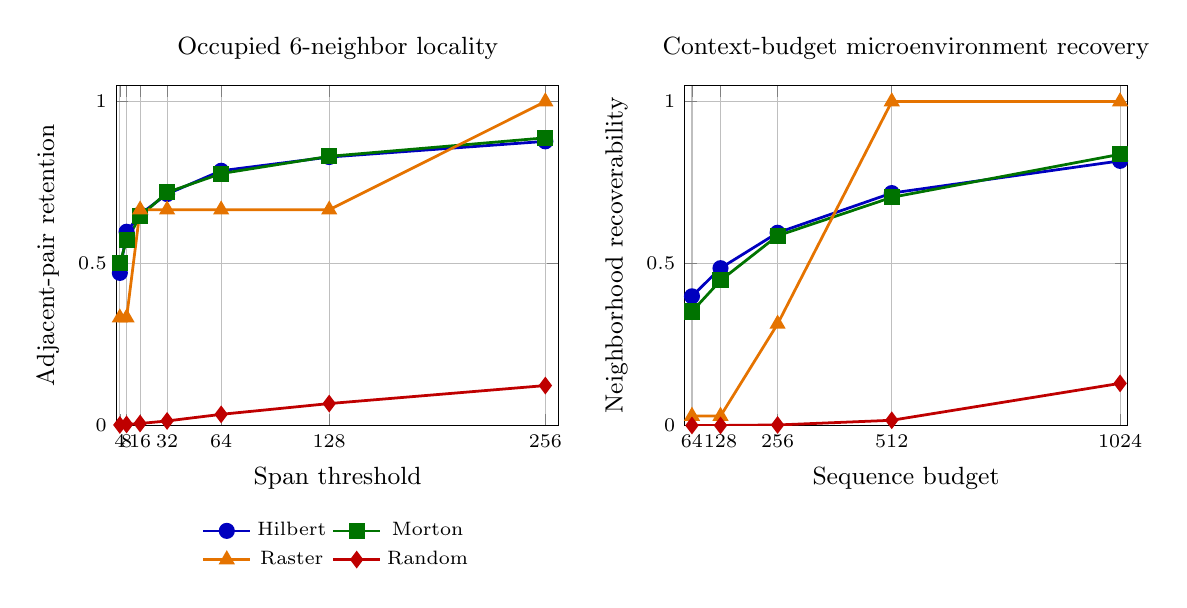
\begin{tikzpicture}
\begin{groupplot}[
  group style={group size=2 by 1, horizontal sep=1.6cm},
]
\nextgroupplot[
  width=7.2cm,
  height=5.9cm,
  xlabel={Span threshold},
  ylabel={Adjacent-pair retention},
  xmin=2,
  xmax=264,
  ymin=0,
  ymax=1.05,
  xtick={4,8,16,32,64,128,256},
  xticklabels={4,8,16,32,64,128,256},
  grid=major,
  tick label style={font=\scriptsize},
  label style={font=\small},
  title style={font=\small},
  title={Occupied 6-neighbor locality},
  legend style={font=\scriptsize, draw=none, at={(0.5,-0.25)}, anchor=north, legend columns=2}
]
\addplot[line width=1.0pt, color=blue!75!black, mark=*, mark size=2.4pt] coordinates {(4,0.4711) (8,0.5981) (16,0.652) (32,0.7145) (64,0.7865) (128,0.8288) (256,0.8773)};
\addplot[line width=1.0pt, color=green!45!black, mark=square*, mark size=2.4pt] coordinates {(4,0.5008) (8,0.5717) (16,0.6455) (32,0.7196) (64,0.7778) (128,0.831) (256,0.8881)};
\addplot[line width=1.0pt, color=orange!90!black, mark=triangle*, mark size=2.4pt] coordinates {(4,0.3325) (8,0.3325) (16,0.666) (32,0.666) (64,0.666) (128,0.666) (256,1.0)};
\addplot[line width=1.0pt, color=red!75!black, mark=diamond*, mark size=2.4pt] coordinates {(4,0.0015) (8,0.0032) (16,0.006) (32,0.0139) (64,0.0343) (128,0.0676) (256,0.1232)};
\addlegendentry{Hilbert}
\addlegendentry{Morton}
\addlegendentry{Raster}
\addlegendentry{Random}

\nextgroupplot[
  width=7.2cm,
  height=5.9cm,
  xlabel={Sequence budget},
  ylabel={Neighborhood recoverability},
  xmin=48,
  xmax=1040,
  ymin=0,
  ymax=1.05,
  xtick={64,128,256,512,1024},
  xticklabels={64,128,256,512,1024},
  grid=major,
  tick label style={font=\scriptsize},
  label style={font=\small},
  title style={font=\small},
  title={Context-budget microenvironment recovery}
]
\addplot[line width=1.0pt, color=blue!75!black, mark=*, mark size=2.4pt] coordinates {(64,0.3988) (128,0.4857) (256,0.595) (512,0.7176) (1024,0.817)};
\addplot[line width=1.0pt, color=green!45!black, mark=square*, mark size=2.4pt] coordinates {(64,0.3518) (128,0.4477) (256,0.5858) (512,0.7044) (1024,0.8373)};
\addplot[line width=1.0pt, color=orange!90!black, mark=triangle*, mark size=2.4pt] coordinates {(64,0.0289) (128,0.0289) (256,0.3133) (512,1.0) (1024,1.0)};
\addplot[line width=1.0pt, color=red!75!black, mark=diamond*, mark size=2.4pt] coordinates {(64,0.0) (128,0.0) (256,0.0015) (512,0.016) (1024,0.13)};
\end{groupplot}
\end{tikzpicture}
\end{document}
